\documentclass[11pt]{beamer}
\usetheme{Madrid}
\usecolortheme{default}

\usepackage[utf8]{inputenc}
\usepackage[italian]{babel}
\usepackage{hyperref}
\usepackage{graphicx}
\usepackage{xcolor}
\usepackage{amsmath}
\usepackage{amsfonts}
\usepackage{amssymb}
\usepackage{subcaption}
\usepackage{appendixnumberbeamer}

\usepackage[ruled,vlined]{algorithm2e}
\SetKwProg{Fn}{Function}{}{}

\definecolor{Sapienza}{RGB}{130, 36, 51}
\setbeamercolor{structure}{fg=Sapienza}
\setbeamercolor{title}{fg=Sapienza}
\setbeamercolor{frametitle}{fg=Sapienza}
\setbeamercolor{title in head/foot}{fg=Sapienza}
\setbeamercolor{author in head/foot}{fg=gray}
\setbeamercolor{date in head/foot}{fg=gray}
\setbeamercolor{section in toc}{fg=Sapienza}
\setbeamercolor{item}{fg=Sapienza}
\setbeamercolor{alerted text}{fg=Sapienza}
\setbeamercolor{block title}{bg=Sapienza, fg=white}
\setbeamercolor{block body}{bg=gray!10}
\setbeamercolor{block title alerted}{bg=Sapienza!80, fg=white}
\setbeamercolor{block body alerted}{bg=Sapienza!5}
\setbeamercolor{block title example}{bg=Sapienza!60, fg=white}
\setbeamercolor{block body example}{bg=Sapienza!5}

\setbeamertemplate{navigation symbols}{}
\setbeamertemplate{footline}[frame number]

\title{NNModelling}
\subtitle{A Visual DSL for Neural Network Design}
\author{Davide Pietragalla \and Luca Sforza}
\institute{Sapienza Universit\`a di Roma}
\date{\today}

\begin{document}

\begin{frame}
	\centering
	
\includegraphics[width=0.5\textwidth]{logoSapienza.png}

	\vspace{10pt}

	{\color{Sapienza} \rule{\textwidth}{0.5mm}}

	\vspace{5pt}

	{\Huge \textbf{Advanced Software Engineering}}

	\vspace{5pt}

	{\color{Sapienza} \rule{\textwidth}{0.5mm}}

	\vspace{25pt}

	{\Huge \color{Sapienza} \textbf{NNModelling}}

	\vspace{10pt}

	{\Large A Visual DSL for Neural Network Design}

	\vspace{10pt}

	{\large Davide Pietragalla \& Luca Sforza}

	\vspace{5pt}

	{\color{gray} \today}
\end{frame}

\begin{frame}{Outline}
	\tableofcontents
\end{frame}

\section{Introduction}

\begin{frame}{Introduction}
	\begin{itemize}
		\item \alert{NNModelling} is a DSL for designing neural network architectures using a visual diagrammatic language
		\item Models are compiled into Hydra configuration files that dynamically instantiate a working \alert{PyTorch Lightning} model
		\item We adopted a \alert{model-driven} approach: UML metamodel $\rightarrow$ front-end editor $\rightarrow$ back-end pipeline
	\end{itemize}

	\vspace{10pt}

	\textbf{Core pipeline}:
	\[
		\text{Visual Graph} \rightarrow \text{NNTree} \rightarrow \text{JSON} \rightarrow \text{Hydra YAML} \rightarrow \text{LightningModule}
	\]
\end{frame}

\section{Requirements}


\begin{frame}{Functional Requirements}

	\alert{Functional Requirements}
	\begin{columns}[t]
		\column{0.5\textwidth}
		\begin{itemize}
			\item Visual Diagram Editor
			\item Node Types (module, input, join, subflow)
			\item Implicit Forks
			\item Explicit Joins
			\item Extensible Module Registry
		\end{itemize}
		\column{0.5\textwidth}
		\begin{itemize}
			\item Subflow Containers
			\item Behavioral Stereotypes
			\item Parameter Configuration
			\item Config Generation
			\item Dynamic Model Instantiation
			\item Training Pipeline
		\end{itemize}
	\end{columns}
\end{frame}



\begin{frame}{Non-Functional Requirements}
	\alert{Non-Functional Requirements}


	\begin{itemize}
		\item \textbf{Separation of Concerns}: front-end handles DSL logic, back-end handles instantiation
		\item \textbf{Test Coverage}: comprehensive tests across both subsystems
		\item \textbf{Expressiveness}: capable of modeling transformers, residual connections, etc.
		\item \textbf{Execution Correctness}: BFS topological traversal with in-degree tracking
	\end{itemize}
\end{frame}

\section{Design}

\begin{frame}{UML Metamodel -- Node Hierarchy}
	\begin{figure}
		\centering
		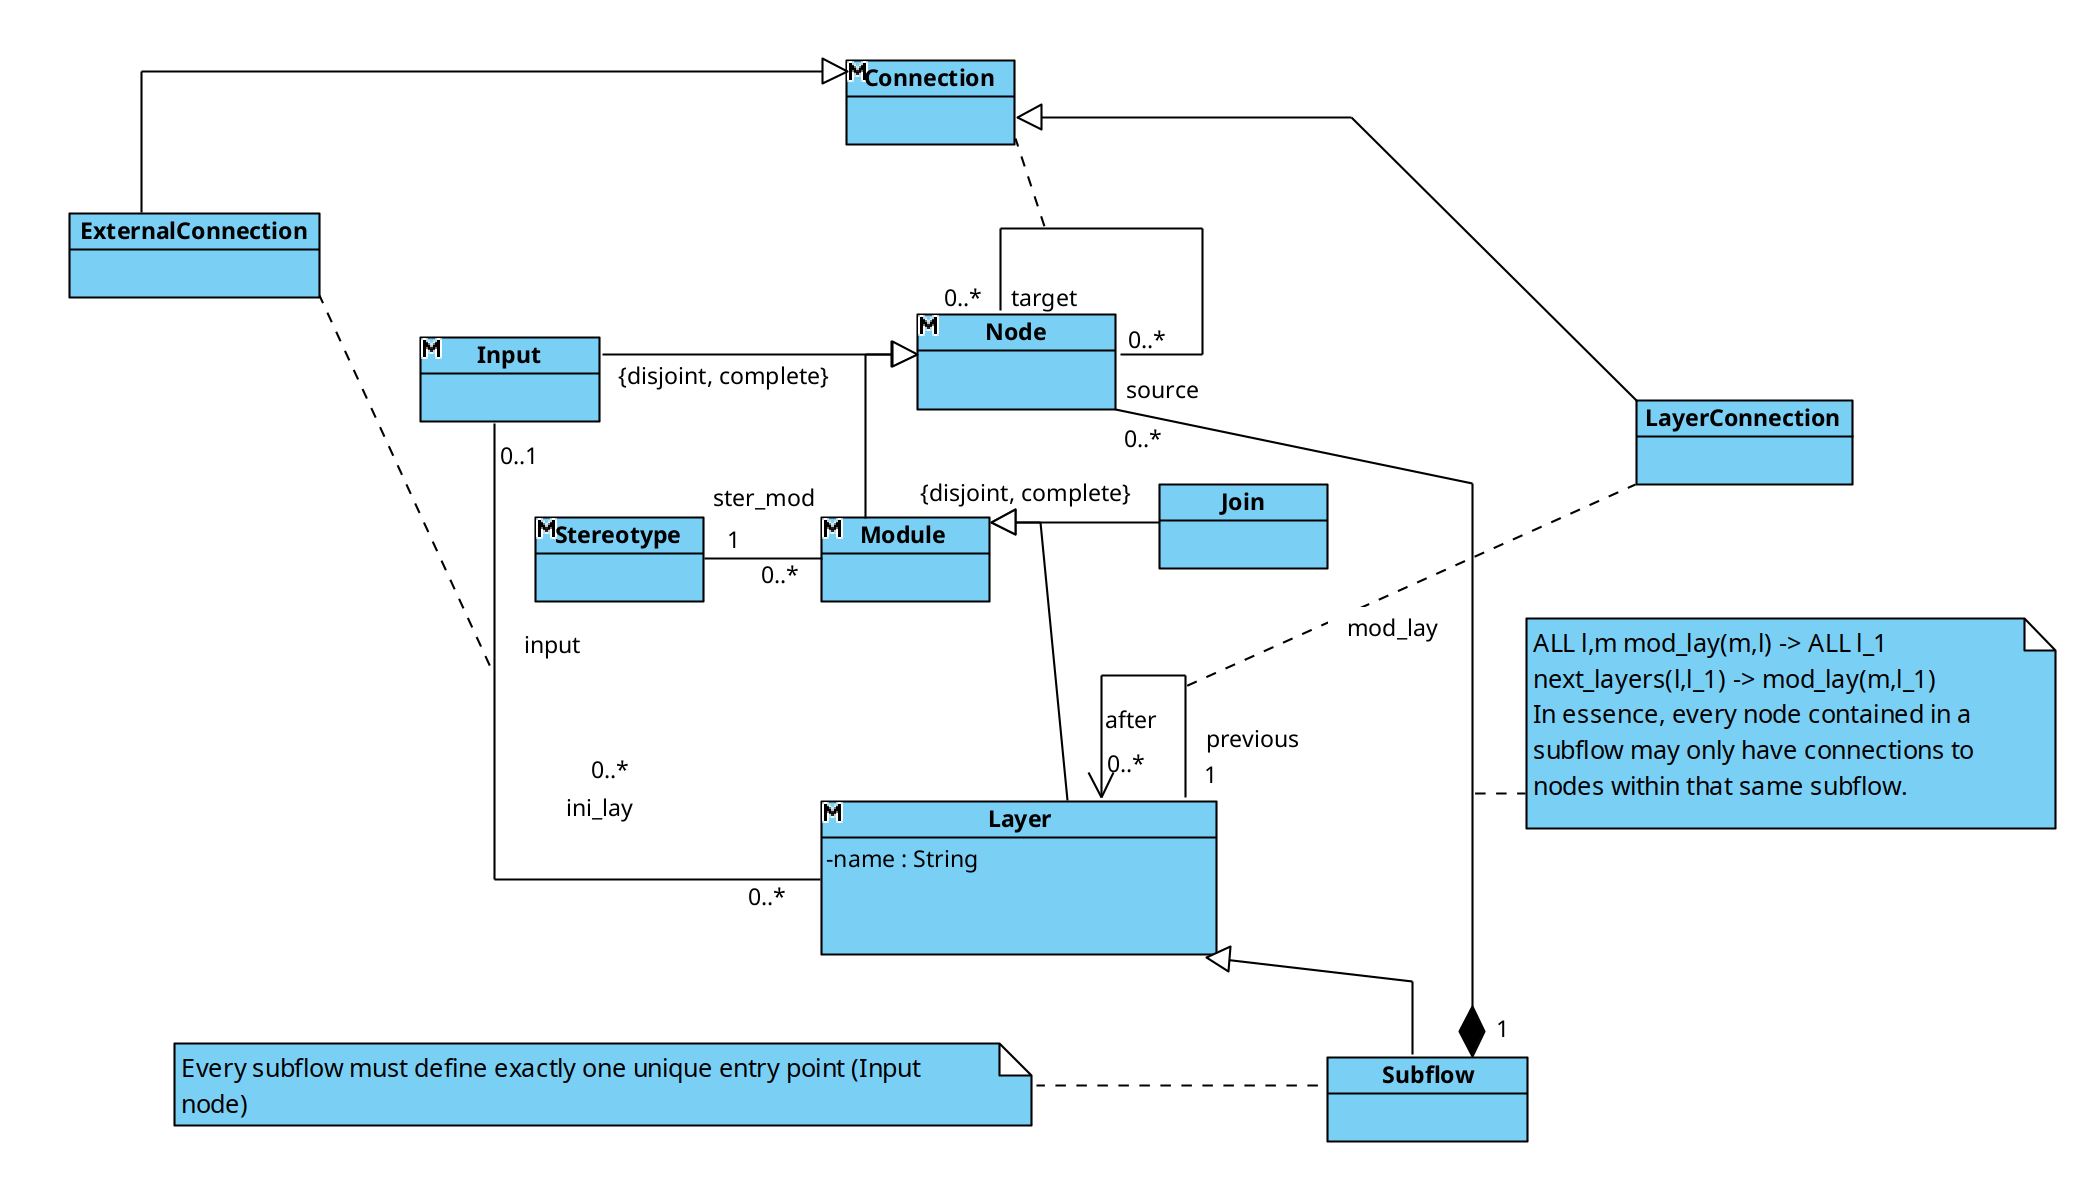
\includegraphics[width=0.85\textwidth]{ModellazioneModules_Layer_Subflow.png}
		\caption{Node hierarchy: Module, Input, Join, Subflow with recursive composition.}
	\end{figure}
\end{frame}

\begin{frame}{UML Metamodel -- Connection Model}
	\begin{figure}
		\centering
		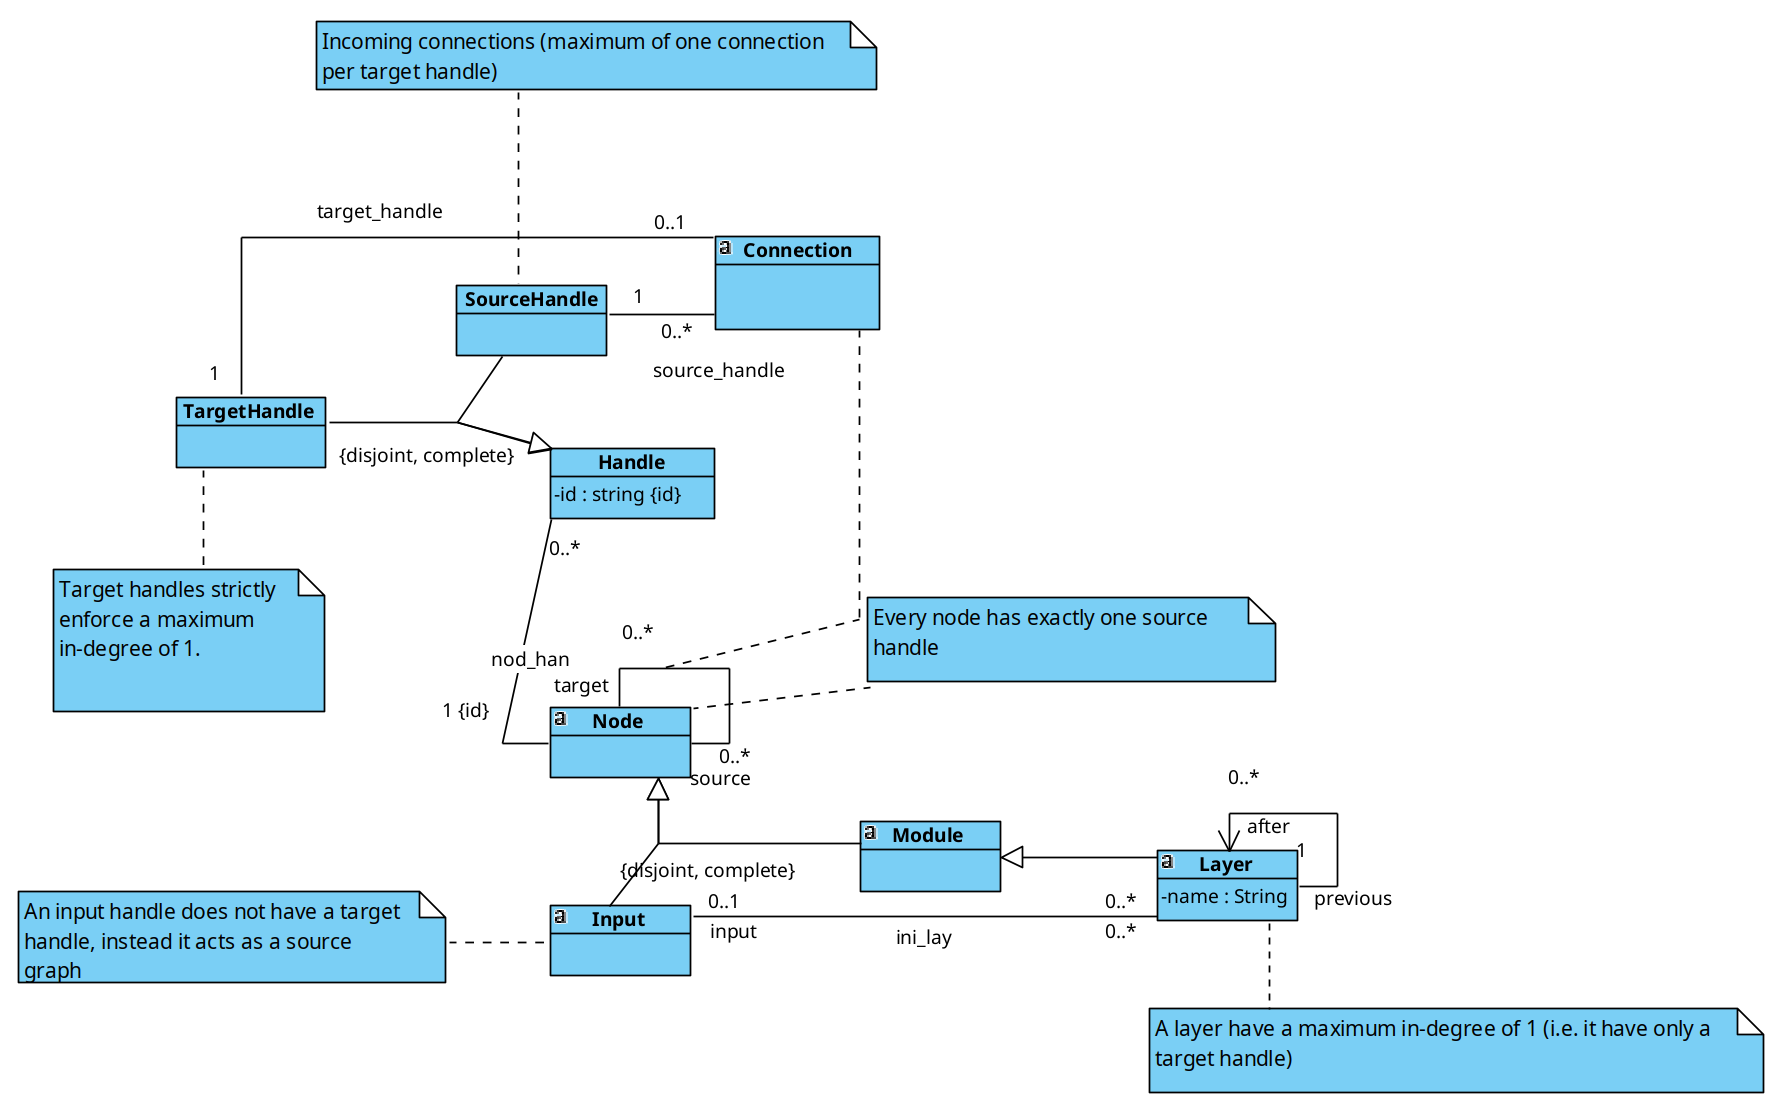
\includegraphics[width=0.85\textwidth]{ModellazioneHandle_E_Node.png}
		\caption{Handle-based connections: implicit forks and explicit joins.}
	\end{figure}
\end{frame}

\begin{frame}{UML Metamodel -- Stereotype System}
	\begin{figure}
		\centering
		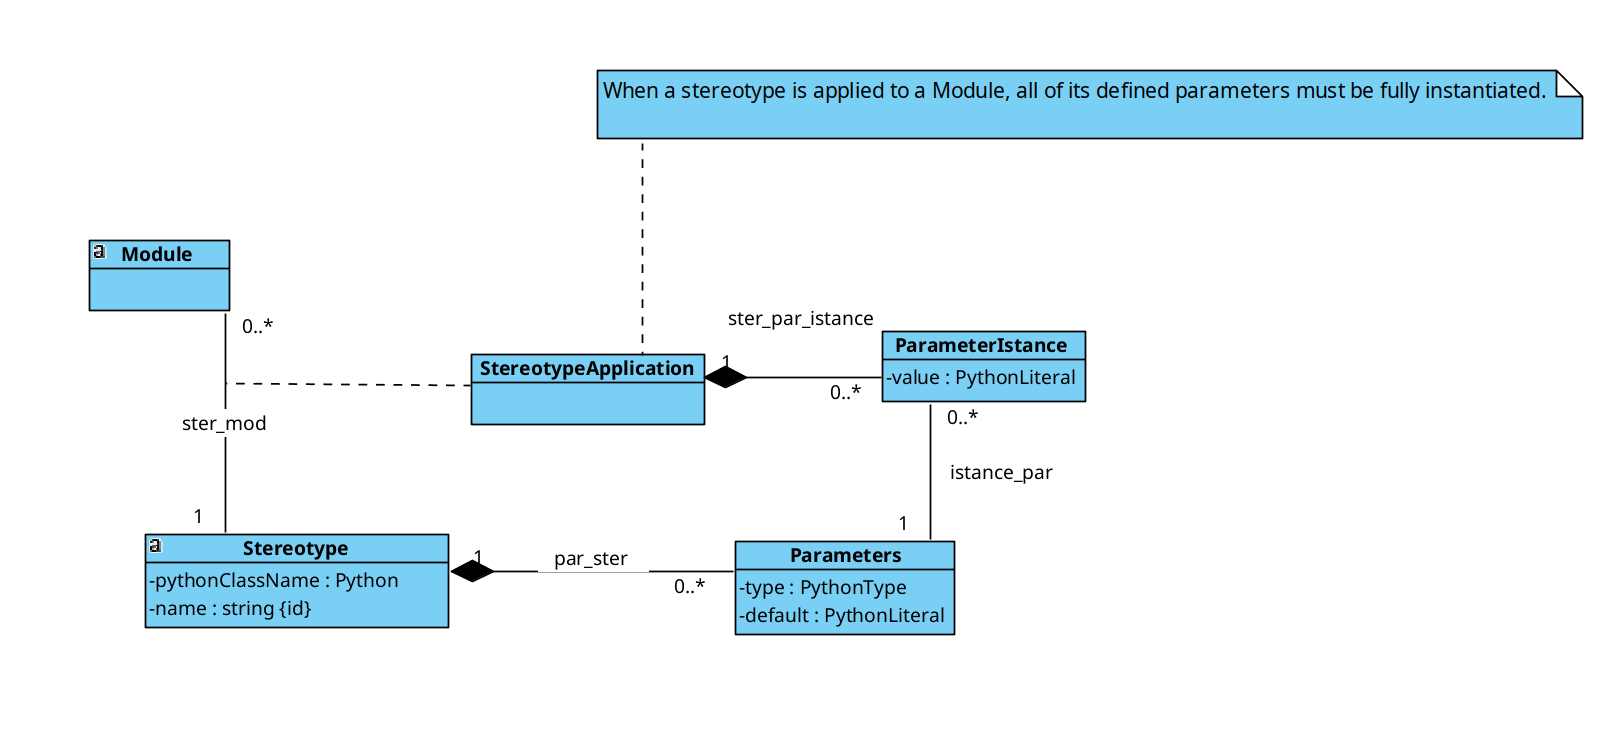
\includegraphics[width=0.85\textwidth]{ModellazioneStereotype_StereotypeIstance_ParameterIstance.png}
		\caption{Stereotype system: separation between definition and instantiation.}
	\end{figure}
\end{frame}

\begin{frame}{Graph-to-NNTree Compilation}
	Formally, a graph $G = (V,E)$ is compiled into a tree $T = (N,C)$

	\vspace{10pt}
	\textbf{Transformations}:
	\begin{itemize}
		\item Maximal linear chains $\rightarrow$ \texttt{Sequential}
		\item Merge points ($indegree > 1$) $\rightarrow$ \texttt{Join}
		\item Subflows $\rightarrow$ recursive compilation
		\item Loss nodes $\rightarrow$ stored separately
	\end{itemize}

	\vspace{10pt}
	Result: an \alert{execution-oriented} representation independent of any DL framework
\end{frame}

\section{Implementation}

\begin{frame}{System Architecture}
	\begin{columns}[t]
		\column{0.5\textwidth}
		\textbf{Front-End}
		\begin{itemize}
			\item Svelte 5, Svelte Flow, TypeScript
			\item Visual DSL editor (browser-only)
			\item Compiler: graph $\rightarrow$ NNTree $\rightarrow$ JSON
		\end{itemize}

		\column{0.5\textwidth}
		\textbf{Back-End}
		\begin{itemize}
			\item Python, PyTorch Lightning, Hydra
			\item Config generator (7 YAML files)
			\item Dynamic model instantiation
		\end{itemize}
	\end{columns}

	\vspace{10pt}
	Communication via JSON file exchange
\end{frame}

\begin{frame}{Supported Components}
	\begin{itemize}
		\item \textbf{27 modules}: Linear, Conv2d, ReLU, Tanh, Embedding, LayerNorm, Dropout, etc.
		\item \textbf{6 joins}: Addition, Concat, Einsum, MatMul, ScaledDotProduct, MaskedScaledDotProduct
		\item \textbf{2 subflow templates}: Repeat (sequential), HorizontalRepeat (parallel via \texttt{vmap})
		\item \textbf{Custom ops}: PositionalEncoding, SequencePool
	\end{itemize}
\end{frame}

\begin{frame}{Dynamic Model Execution}
	\alert{Dynamic Model Execution}
	\begin{itemize}
		\item The \texttt{Net} class extend \texttt{LightningModule} and it build the architecture from a Hydra config at runtime.
		\item \texttt{forward} method is implemented as a \alert{BFS traversal of the network with in-degree tracking}
		\item Join nodes collect all inputs ordered by \texttt{targetHandle}
		\item Custom operations: Subflow, Repeat, HorizontalRepeat
	\end{itemize}
	\vspace{10pt}
\end{frame}

\section{Validation}

\begin{frame}{Example: Transformer Classifier}

	\alert{Example: Transformer Classifier}

	Three-level Flow for Building the Encoder:

	\begin{itemize}
		\item \small Top-level: Input $\rightarrow$ Embedding $\rightarrow$ PosEnc $\rightarrow$ Transformer $\rightarrow$ Pool $\rightarrow$ Linear $\rightarrow$ Loss
		\item \small Repeat encoder with residual blocks and FFN
		\item \small HorizontalRepeat multi-head attention with Q/K/V projections
	\end{itemize}
	The architecture is taken from "Attention Is All You Need" paper.

	\vspace{10pt}
	\textbf{Result}: 98.4\% accuracy on EnronSpam test set.
\end{frame}

\begin{frame}{Training Metrics}
	\begin{figure}
		\centering
		\begin{subfigure}{0.45\textwidth}
			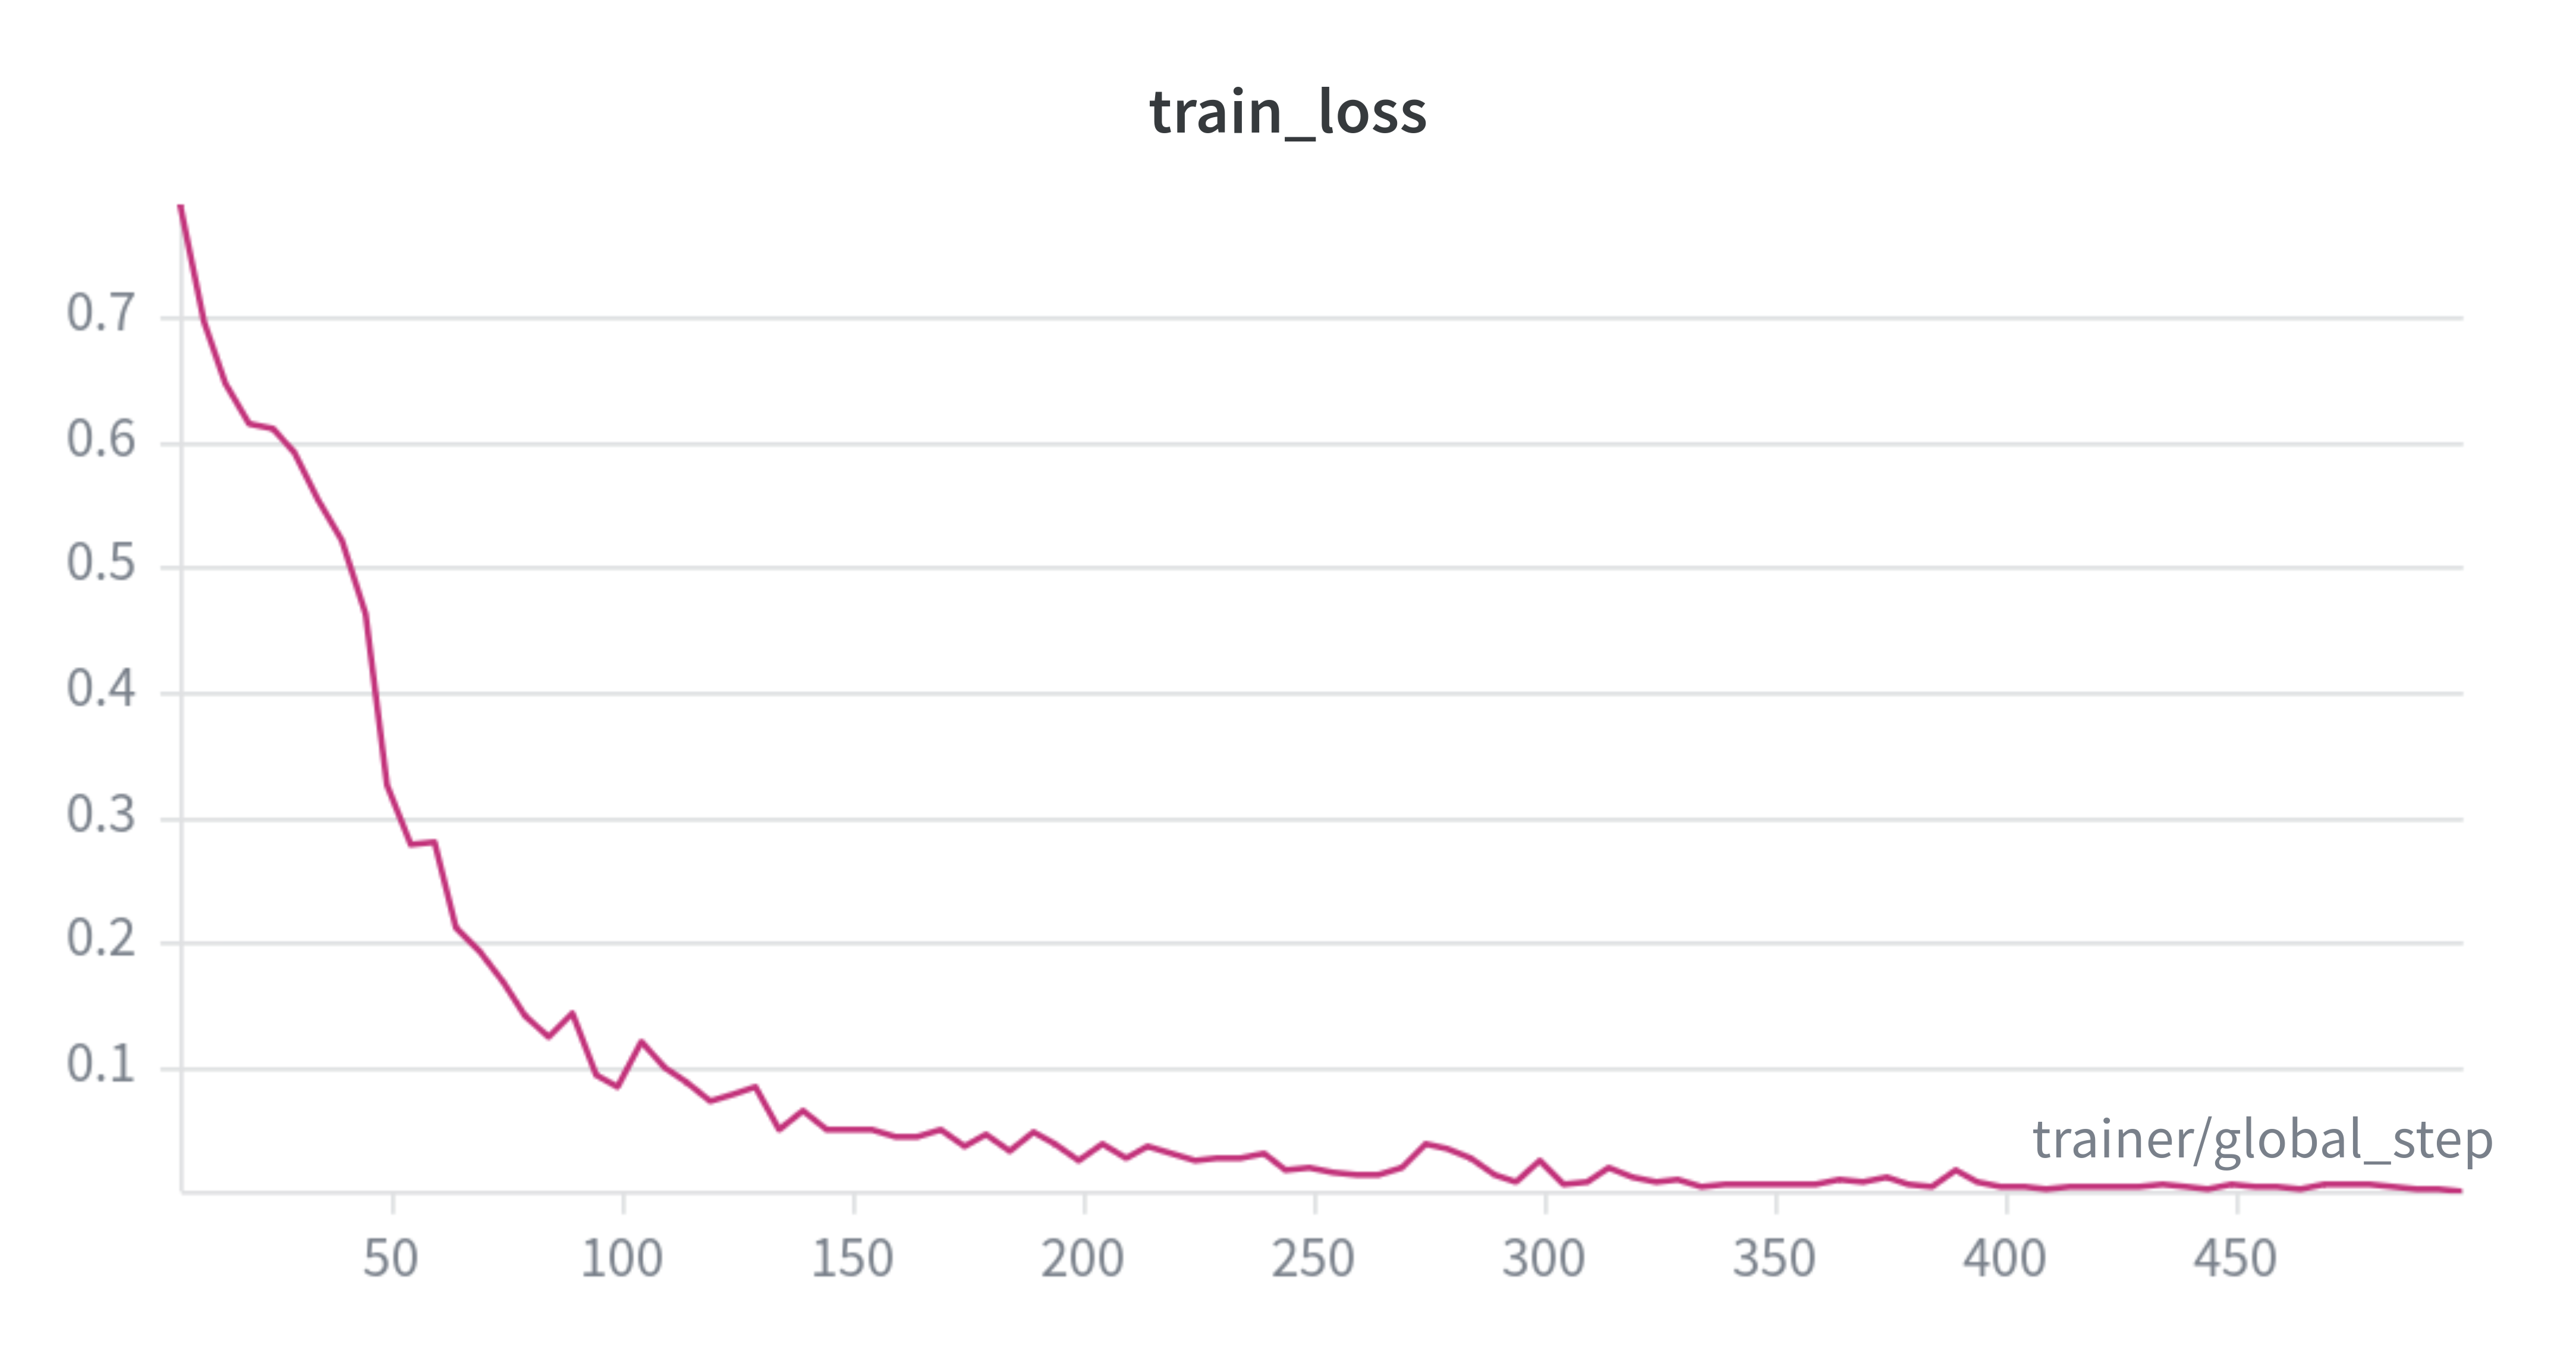
\includegraphics[width=\textwidth]{train_loss.png}
			\caption{Training loss}
		\end{subfigure}
		\hfill
		\begin{subfigure}{0.45\textwidth}
			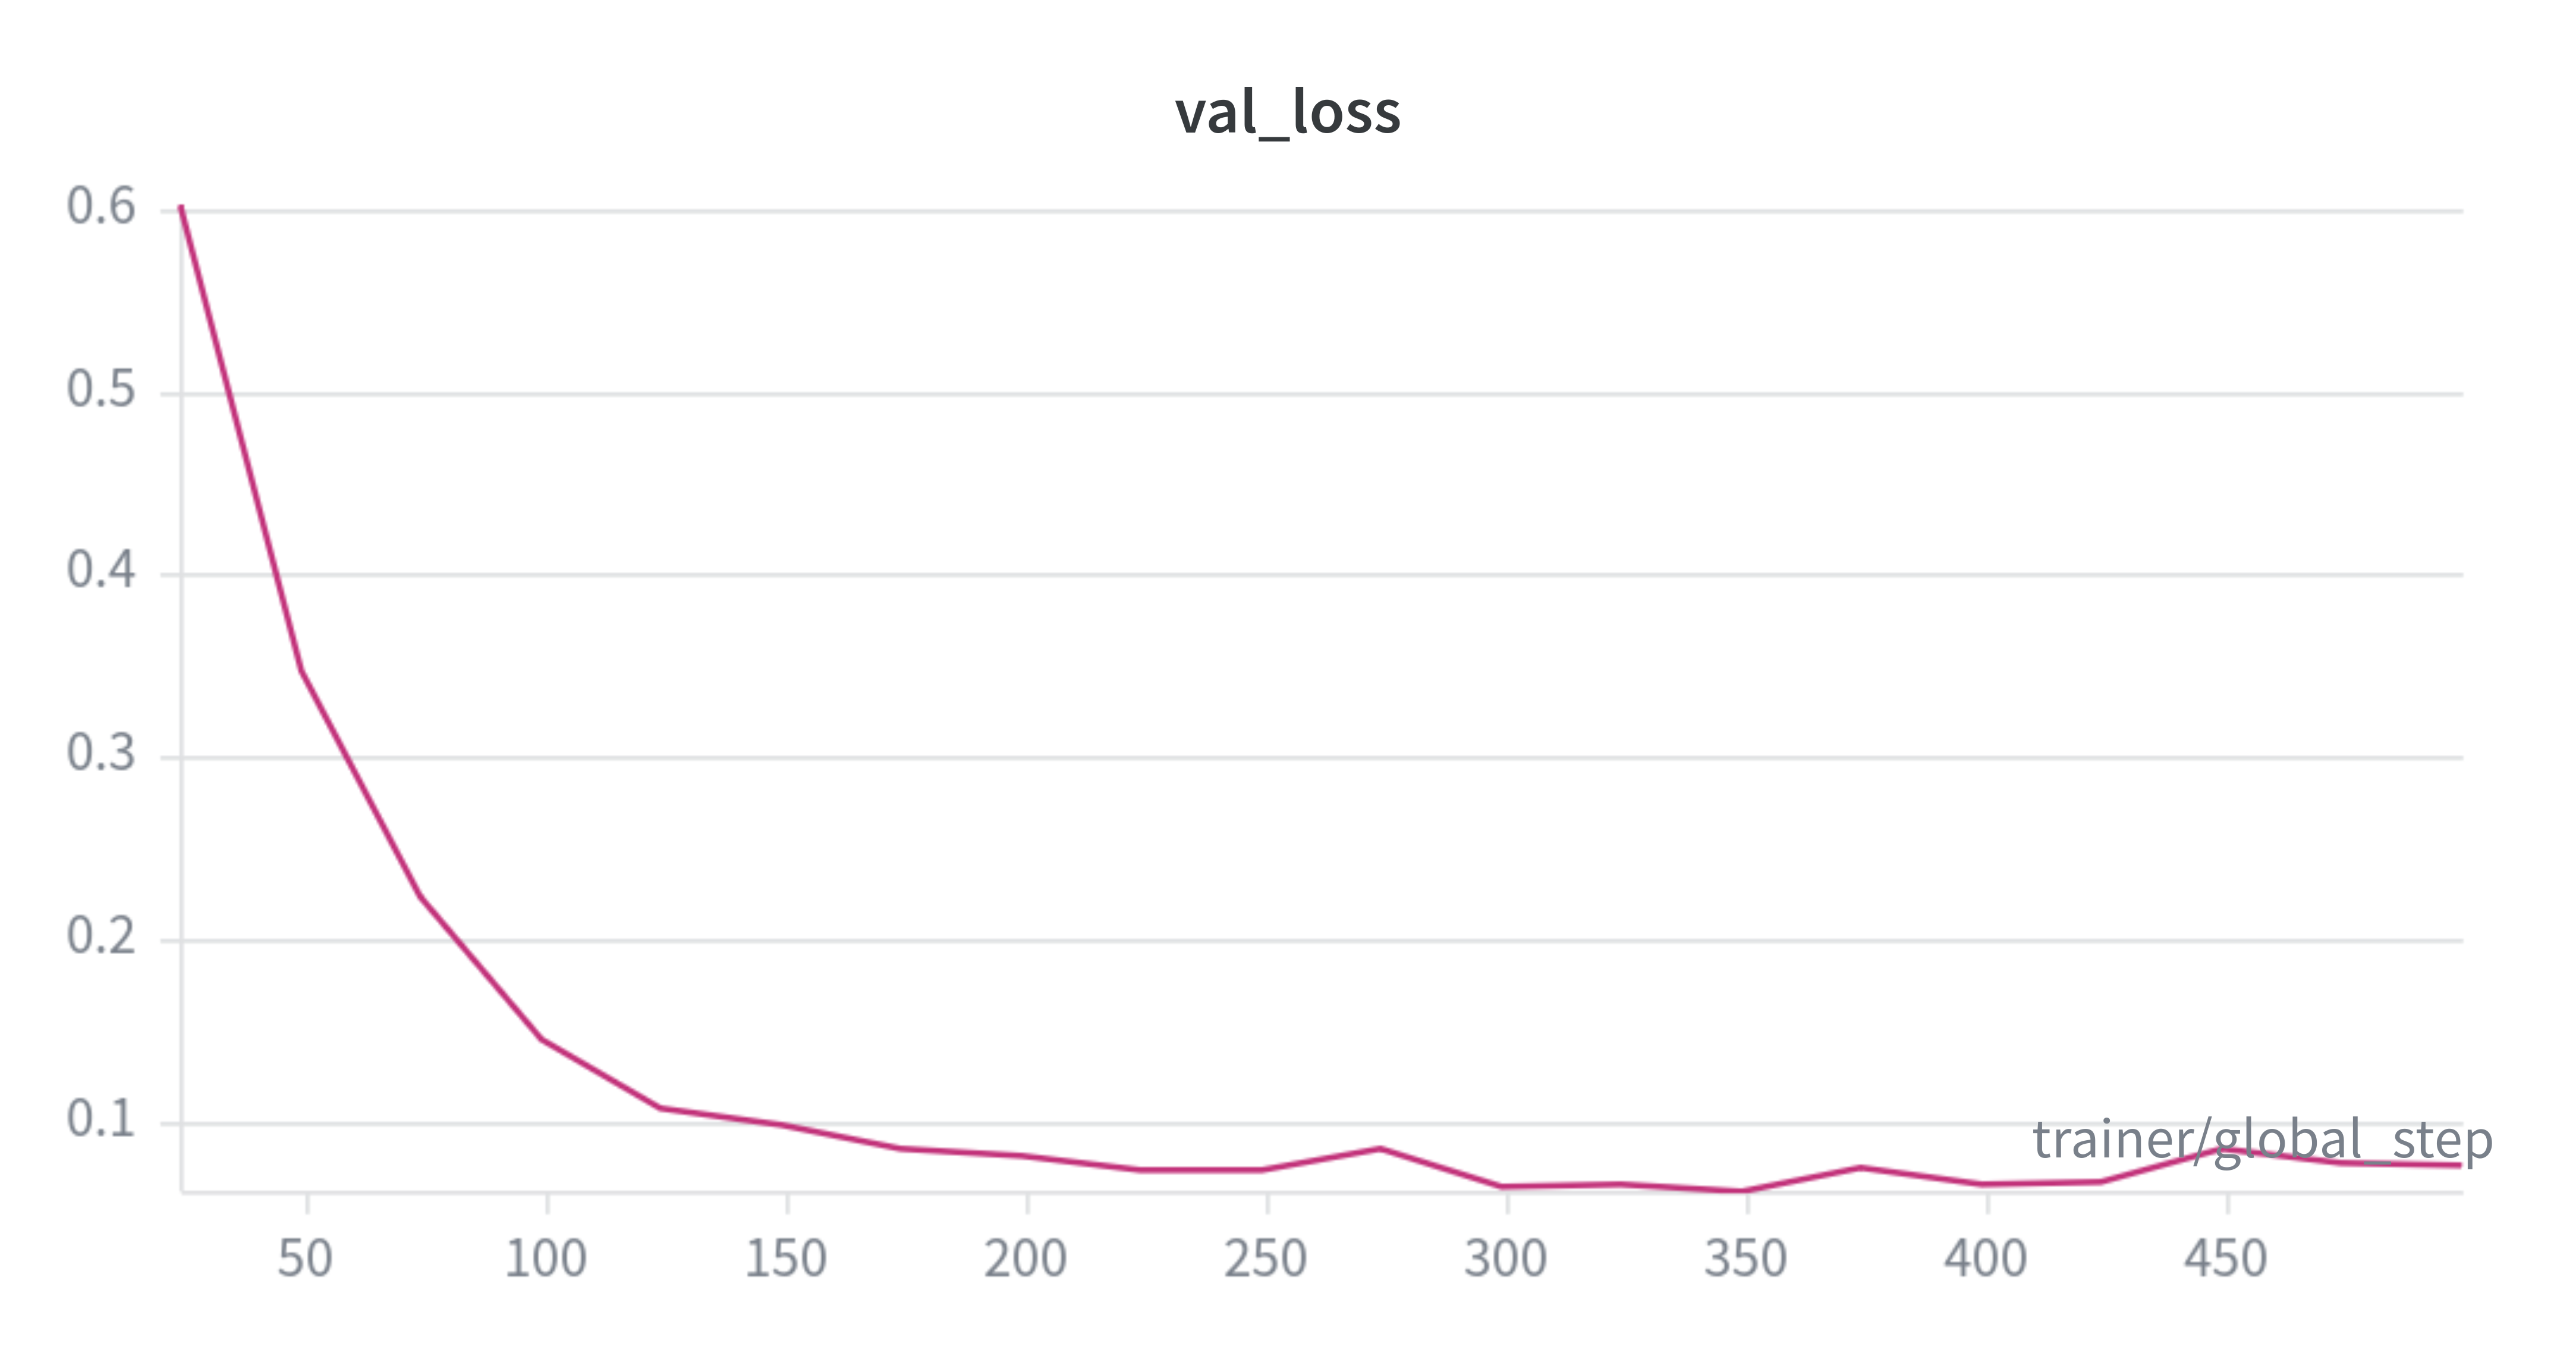
\includegraphics[width=\textwidth]{val_loss.png}
			\caption{Validation loss}
		\end{subfigure}

		\vspace{10pt}

		\begin{subfigure}{0.45\textwidth}
			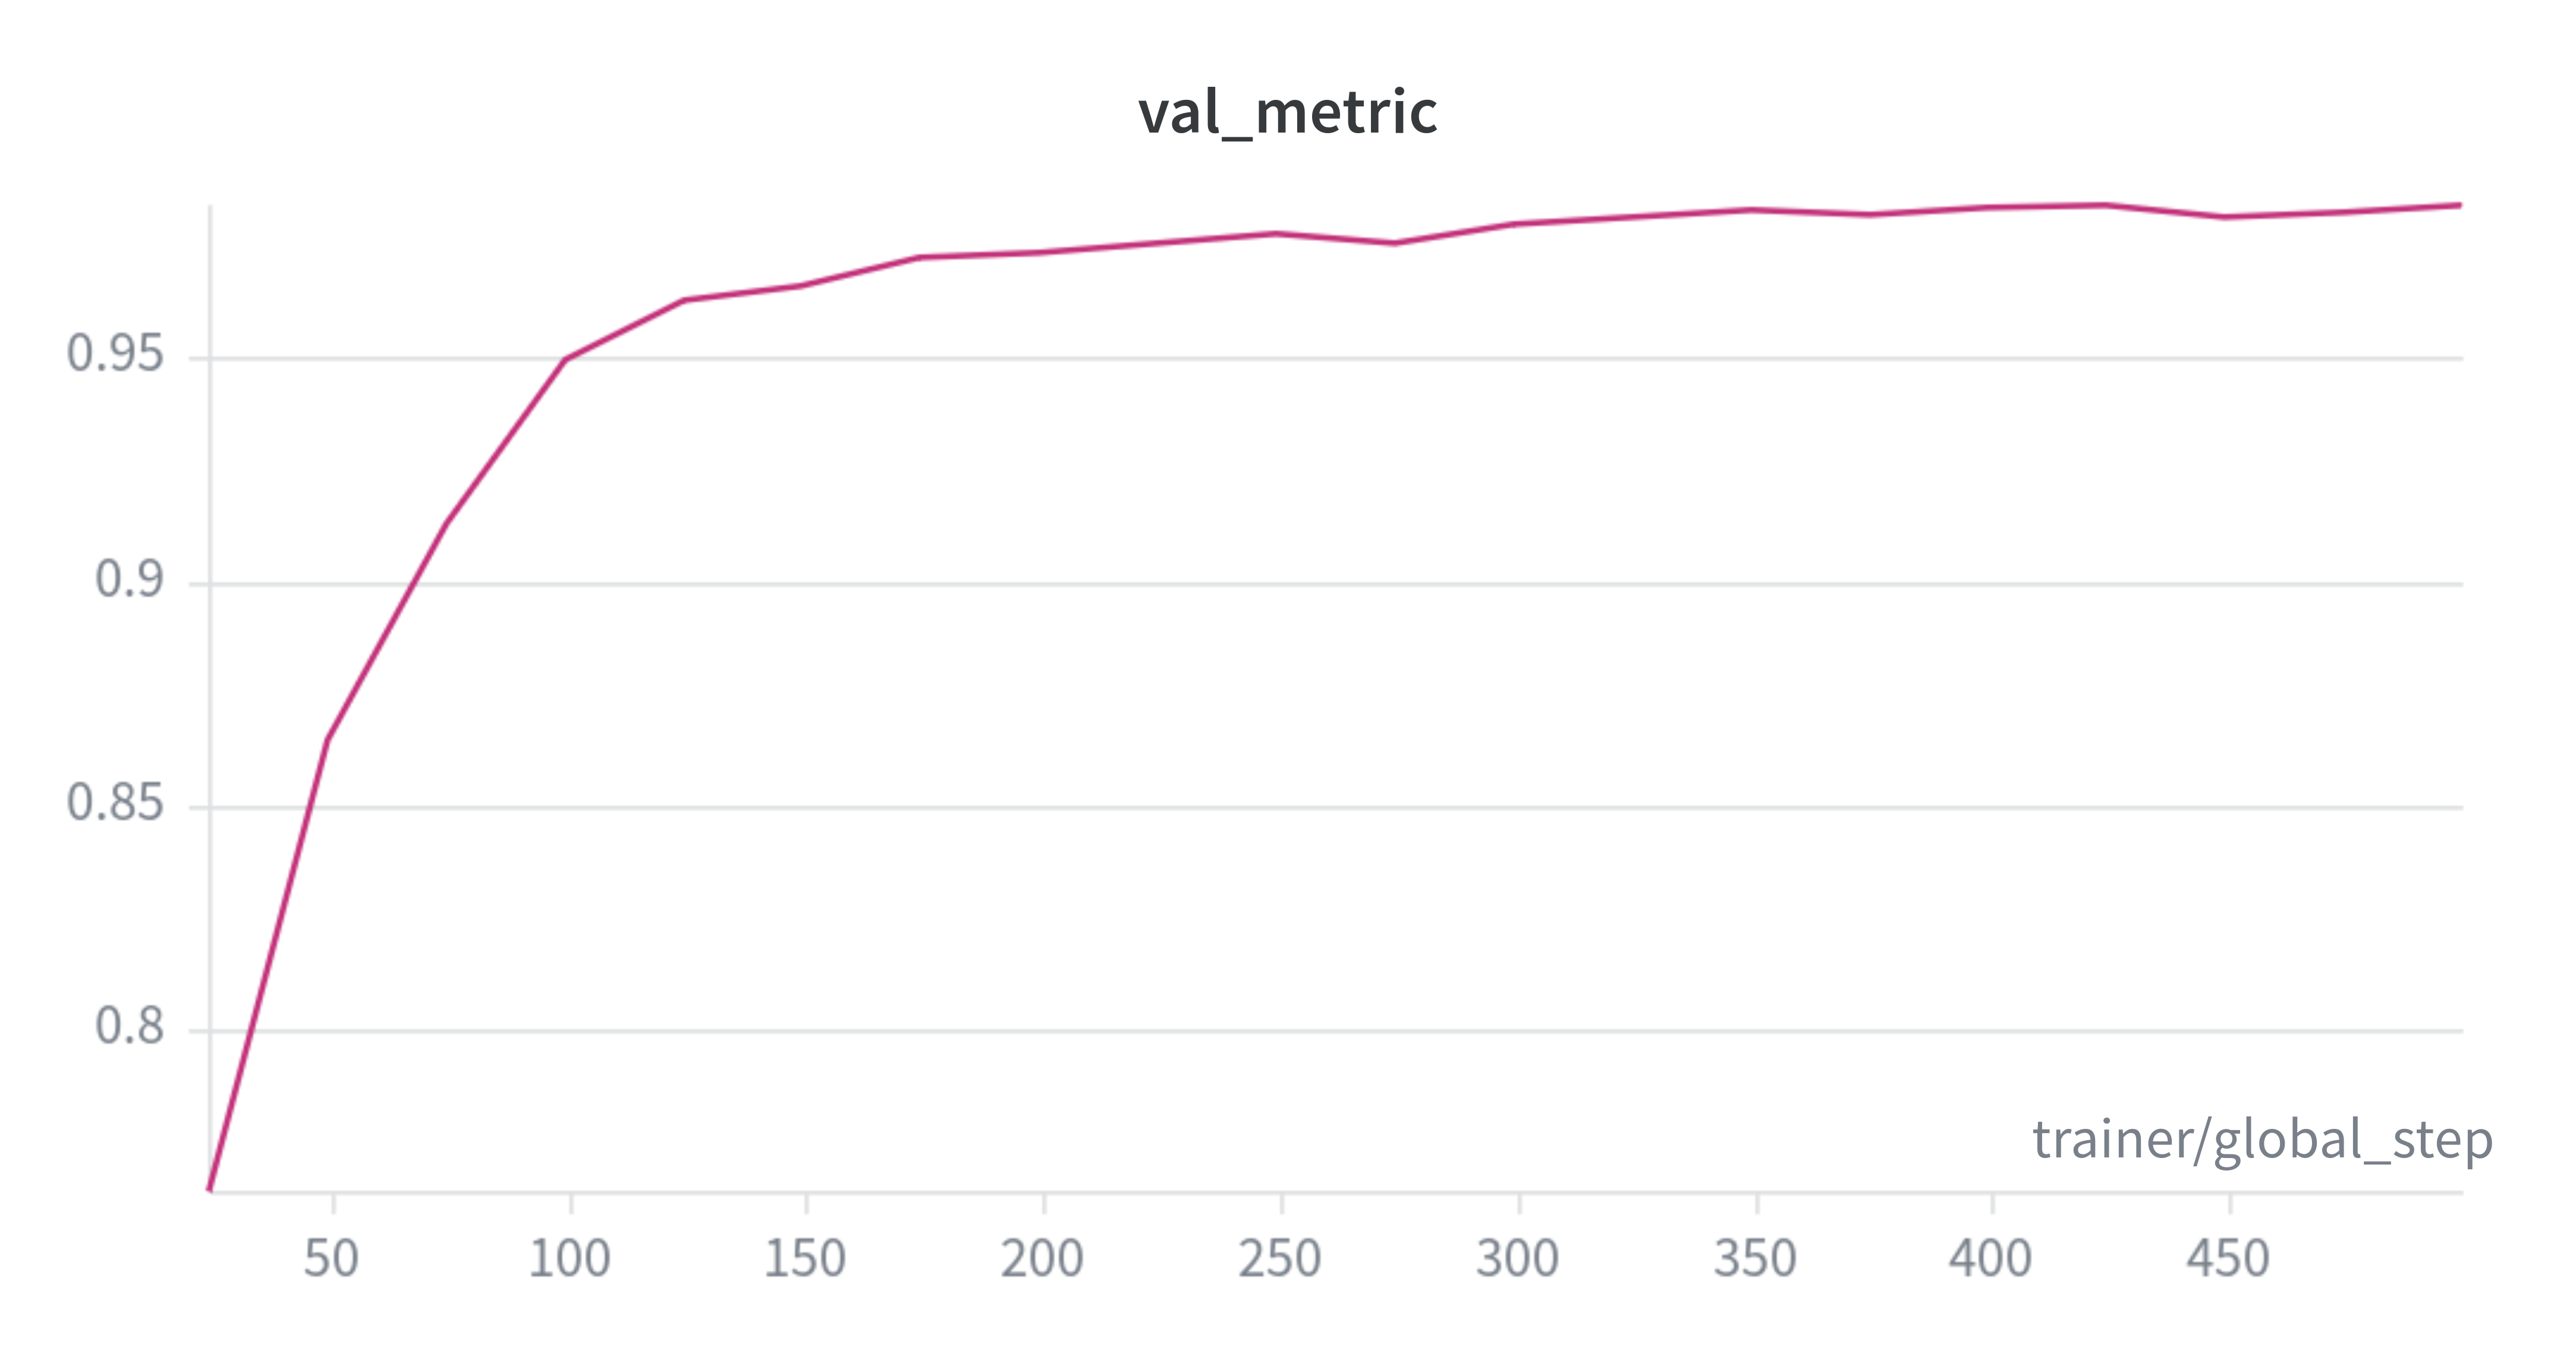
\includegraphics[width=\textwidth]{val_metric.png}
			\caption{Validation accuracy}
		\end{subfigure}
	\end{figure}
\end{frame}

\section{Conclusions}


\begin{frame}{Achievements}

	\alert{Achievements}
	\begin{itemize}
		\item Full \alert{end-to-end pipeline} from visual design to trained model
		\item Extensible \alert{stereotype system} -- no code changes for new layers
		\item Complex architectures: transformers, residual nets, subflows
		\item \alert{179 tests} ensuring reliability
		\item Model-driven approach for the develoment process
		\item Clean \alert{separation of concerns}
	\end{itemize}
\end{frame}

\begin{frame}{Future Work}

	\alert{Future Work}
	\begin{itemize}
		\item \alert{Network Communication}: replace file exchange with HTTP/WebSocket API
		\item \alert{Configurable Join}: parameterize HorizontalRepeat merge strategy
		\item \alert{Parallel Execution}: CUDA stream dispatcher for fork-join topologies
		\item \alert{Subflow Persistence}: save/load subflows independently
		\item \alert{Interactive Deployment}: HuggingFace Spaces
		\item \alert{Pre-trained Models}: transfer learning support
	\end{itemize}
\end{frame}

\appendix

\begin{frame}{Transformer Architecture}
	\begin{figure}
		\centering
		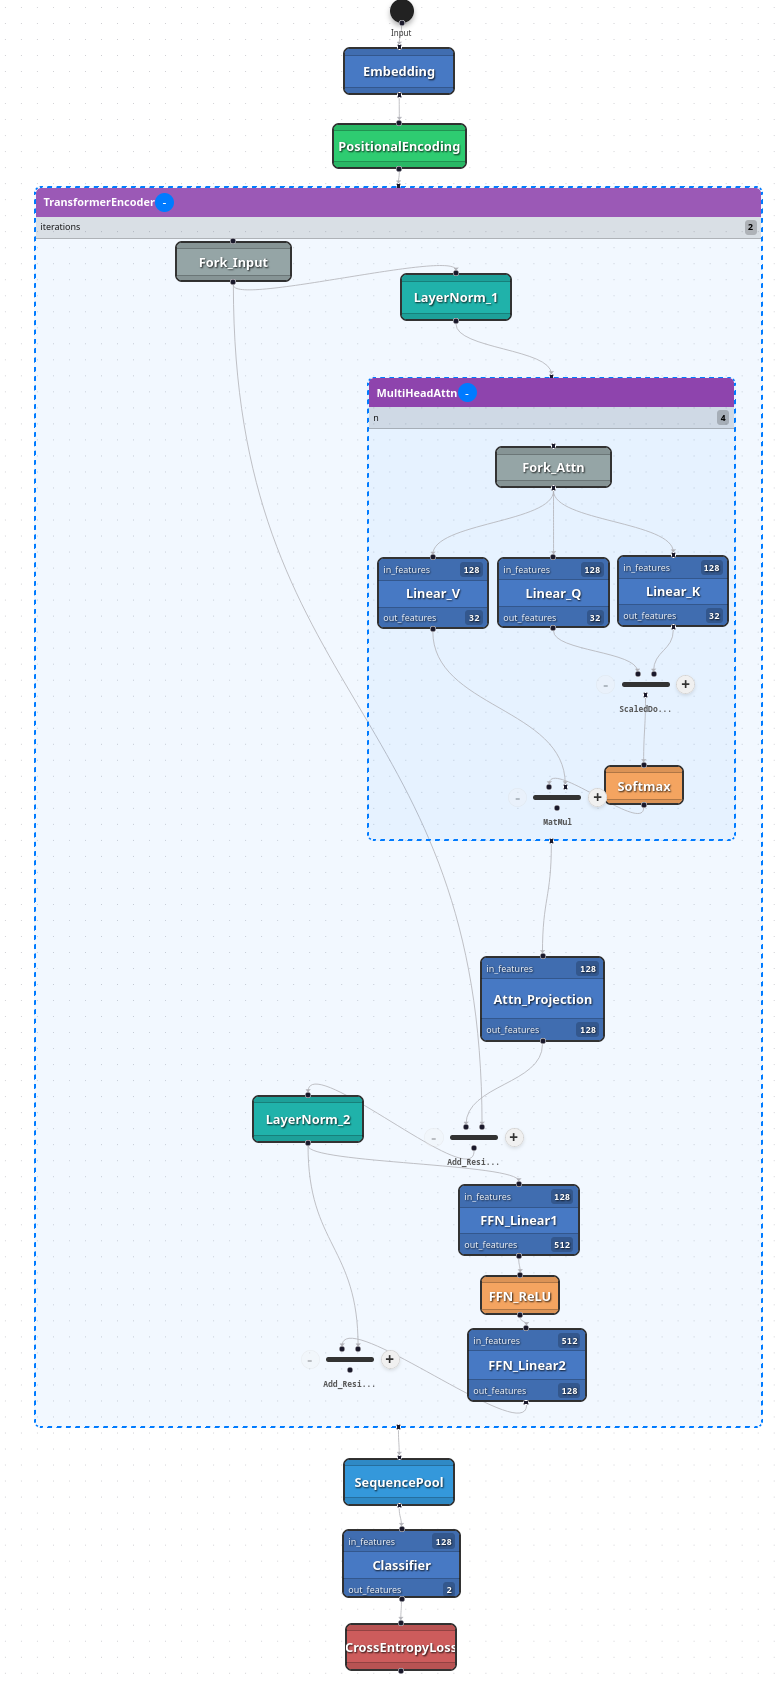
\includegraphics[width=0.85\textwidth,height=0.75\textheight,keepaspectratio]{transformer_classifier_diagram.png}
		\caption{Full transformer classifier graph in the NNModelling editor}
	\end{figure}
\end{frame}

\begin{frame}{References}
	\begin{thebibliography}{5}
		\bibitem{svelte5} Svelte 5 Documentation. \url{https://svelte.dev/docs}
		\bibitem{svelteflow} Svelte Flow Documentation. \url{https://svelteflow.dev/}
		\bibitem{pytorch} Paszke, A. et al. ``PyTorch: An Imperative Style, High-Performance Deep Learning Library.'' NeurIPS 2019.
		\bibitem{lightning} Falcon, W. et al. ``PyTorch Lightning.'' \url{https://lightning.ai/}
		\bibitem{attention} Vaswani, A. et al. ``Attention Is All You Need.'' NeurIPS 2017.
		\bibitem{hydra} Yadan, O. ``Hydra - A Framework for Elegantly Configuring Complex Applications.'' \url{https://hydra.cc/}
	\end{thebibliography}
\end{frame}

\end{document}
